%_____________________________________________________________________________________
%
%       Filename:  chapter2.tex
%
%    Description:  Thesis Template HS Offenburg
%
%
%         Author:  Okba ZOUEGHI, okba.zoueghi@gmail.com
%     Supervisor:  Andreas Walz, Chadlia Jerad
%   Organization:  HS Offenburg, Offenburg, Germany
%
%_____________________________________________________________________________________

\chapter{State of the art}
\label{chap:chapter2}

Using one of the available security protocols, our project aims to secure SafetyNETp \ac{RTFN} based communication.
Therefore an overview and a description of those concepts are required. As SafetyNETp is an Industrial network protocol, we start the chapter with an overview of the history of industrial networks, then
we introduce SafetyNETp protocol and its communication models. Finally, we go through an overview of
the security protocols to choose the suitable one for our project.


\section{Industrial Networks} % (fold)
Nowadays we could not imagine a world without emails, online newspapers, blogs,
chat and the other services offered by the internet.
All these services are made possible thanks to the development of networking.
Networking plays an important role not only in our daily lives but also in
manufacturing and process automation. Unlike the networks that we are used to
in our daily lives, where devices like mobile phones, TVs, printers, and
computers are interconnected, in the industry, other types of devices are
interconnected such as sensors, motors, actuators, robots and similar other
devices. Hence we can speak about industrial networks.

The industrial systems faced the needs for improvement in production
monitoring and quality control and at the same time maintaining
the costs of all this as low as possible. This happened in the
last few decades due to the growth of social needs, which in turn enforce
the industrial systems to grow to match up with these needs.
So any operation that runs manually had to be replaced with a faster, and more
reliable automated operation. This provides the factories with
the necessary monitoring which allows better supervisory and quality control.
Introducing all this number of automated units into the factories needed an efficient
method to connect them together, to communicates with each other, and to transfer the
various supervisory data to the monitors.

Ethernet and Fieldbus are the two big keywords when it comes to industrial communication systems.
In this section, we go into an overview in which we see the evolution
of the industrial networks across the time \cite{zurawski2014industrial}.



% \subsection{Fieldbus systems}
%
% The word Fieldbus is basically the combination of two terms, field and bus.
% The meaning behind field as defined in the industrial word is a geographical area or space in which the industrial instruments such as sensors and actuators are situated and working. These industrial instruments' tasks are performed in the field level, hence they are commonly called field devices.
%  Regarding the term bus, in computer science, it refers to a line
% which allows connecting several units and permits to transfer
% data through it. Before going more into Fieldbus systems, let's
% see first how was the industrial networks before their introduction \cite{zurawski2014industrial}.
%
%
%
% In the industrial world like it shows the \autoref{Centralized_point-to-point_architecture}, the first solution that has been used for connecting field devices
% was parallel wiring or in other words star topology \cite{zurawski2014industrial}. Every field device is wired
% to a control computer which performs the control and the monitoring tasks. In order to perform these tasks, the
% control computer needs to transfer the data back and forth from the field devices using the traditional
% point-to-point technology. This architecture presents several
% disadvantages, it demands a high cost because of the point-to-point wiring, every field device needs to be wired
% separately to the control computer, moreover, If this control computer goes down all the system will collapse.
%
% \begin{figure}
% \centering
% 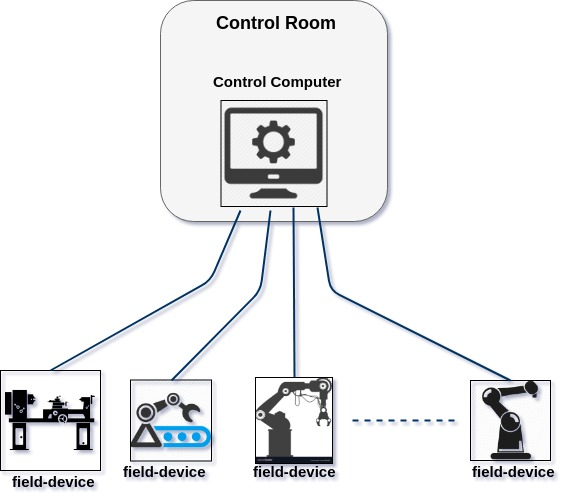
\includegraphics[width=12cm,height=8cm]{figures/fieldbus/star_topology_used_up_to_1960.jpg}
% \caption{Centralized point-to-point architecture}\label{Centralized_point-to-point_architecture}
% \end{figure}
%
% As a second step, unlike the previous solution which relies on a centralized control, In order to reduce the system fault,
% the new architecture includes more than one control computer \cite{zurawski2014industrial}. Each control computer controls and supervises a group
% of field devices, hence the risk of system fault is decreased. The \autoref{Decentralized_point-to-point_architecture}
% shows an example of a decentralized architecture.
%
% \begin{figure}
% \centering
% 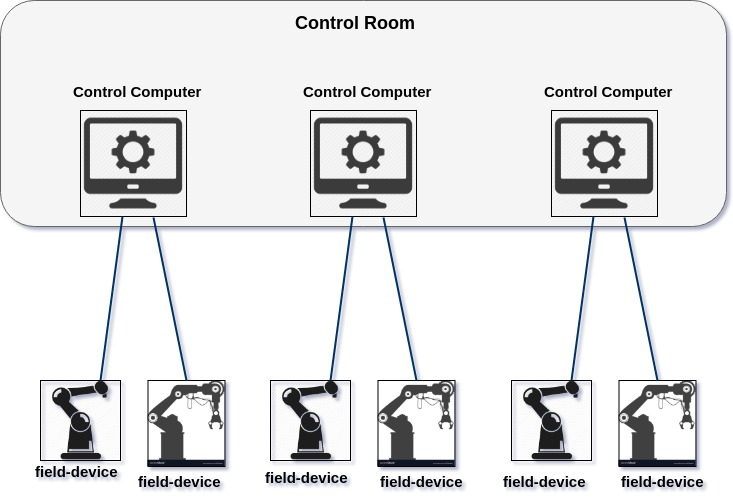
\includegraphics[width=12cm,height=8cm]{figures/fieldbus/decentralized_topology.jpg}
% \caption{Decentralized point-to-point architecture}\label{Decentralized_point-to-point_architecture}
% \end{figure}
%
% Each step aims to reduce the costs compared with the previous one. After the decentralization of control devices, In order to reduce
% the wiring cost, a local control-device is installed next to each group of field devices \cite{zurawski2014industrial}. As
% shown in \autoref{Local_control_devices} each one of the control-devices controls and monitors a group of filed-devices. These
% control-devices are then wired to a central supervisory computer. This solution keeps the advantages of the
% previous ones, in addition, it significantly reduce the length of the wires which eventually reduce the cost with an important manner.
%
% \begin{figure}
% \centering
% 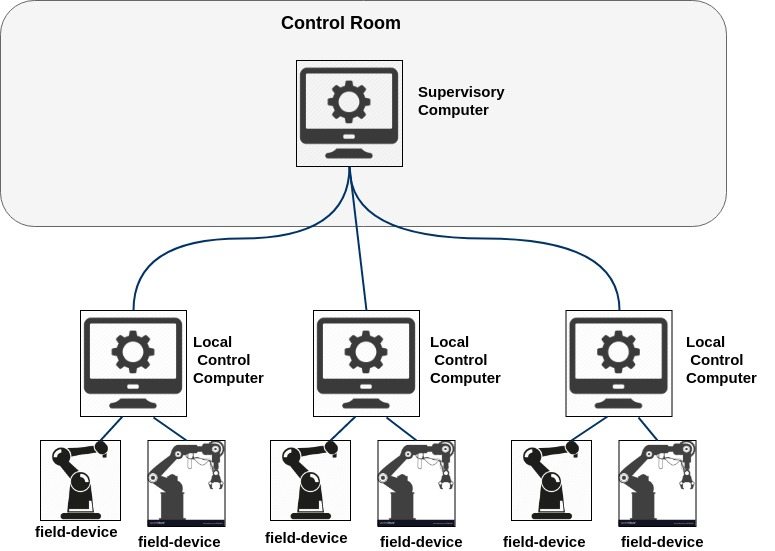
\includegraphics[width=12cm,height=7cm]{figures/fieldbus/local_control_devices.jpg}
% \caption{Local control devices}\label{Local_control_devices}
% \end{figure}
%
% After all this evolution, the point-to-point wiring problem is still present. The solution was the famous Fieldbus systems.
% The desire to cope with the wiring problem getting out of hand in large installations was certainly the main impetus for its development.
% Fieldbus systems were introduced in 1980 and the idea behind them is to connect all the field devices with one single link called Fieldbus \cite{zurawski2014industrial}.
% To be able to let all the field devices communicate and transfer data through one single line, a communication protocol should be used
% to manage the bus access. The communication protocol will be responsible to define a mechanism for acquiring the bus and devices synchronization.
% Hence the data transferred through the bus will be multiplexed in time. An example of a protocol that can be used for managing the Fieldbus access, the
% \ac{CSMA} protocol. The advantages introduced by the Fieldbus systems are many, the most important is the substantial reduction of wiring
% and adding more flexibility. With Fieldbus systems, the network extension is very much easier to achieve.
% For instance, CAN is one of the most well-known Fieldbus systems. It is mostly used in automotive networks.
% The \autoref{fieldbus_network} shows the architecture of a Fieldbus network.
%
% \begin{figure}
% \centering
% 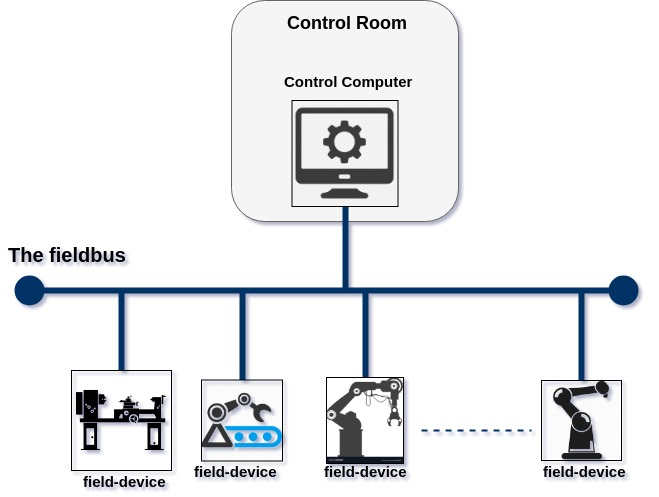
\includegraphics[width=12cm,height=7cm]{figures/fieldbus/fieldbus_network.jpg}
% \caption{Fieldbus network}\label{fieldbus_network}
% \end{figure}

\subsection{Fieldbus Systems}

The word Fieldbus is basically the combination of two terms, field and bus.
The meaning behind field as defined in the industrial world is a geographical
area or space in which the industrial instruments such as sensors and actuators
are situated and working. These industrial instruments' tasks are performed at the
field level, hence they are commonly called field devices.
Regarding the term bus, in computer science, it refers to a line
which allows connecting several units and permits to transfer
data through it. Before going more into Fieldbus systems, let's
see first how was the industrial networks before their introduction \cite{zurawski2014industrial}.

In the industrial world, as shown in \autoref{Centralized_point-to-point_architecture}, the first solution
that has been used for connecting field devices
was star topology \cite{zurawski2014industrial}. Every field device is wired
to a control computer which performs the control and the monitoring tasks. In order to perform these tasks, the
control computer needs to transfer the data back and forth from the field devices using the traditional
point-to-point technology. This architecture presents several
disadvantages, it demands a high cost because of the point-to-point wiring, every field device needs to be wired
separately to the control computer, moreover, if this control computer goes down, all the system will collapse.

\begin{figure}[!htbp]
\centering
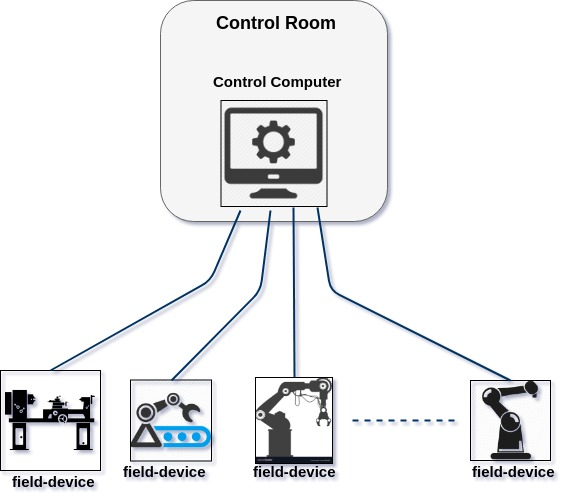
\includegraphics[width=9cm]{figures/fieldbus/star_topology_used_up_to_1960.jpg}
\caption{Centralized point-to-point architecture}\label{Centralized_point-to-point_architecture}
\end{figure}

The desire to cope with the wiring problem getting out of hand in large installations was certainly the main impetus
for the development of Fieldbus systems. Fieldbus systems were introduced in 1980 and the idea behind them is to connect all the field
devices with one single link called Fieldbus \cite{zurawski2014industrial}. To be able to let all the field devices
communicate and transfer data through one single line, a communication protocol should be used to manage the bus
access. The communication protocol is responsible for defining a mechanism for acquiring the bus.
Hence the data transferred through the bus will be multiplexed in time. An example of a protocol that can be used for
managing the Fieldbus access is the \ac{CSMA} protocol. The advantages introduced by the Fieldbus systems are many, the most
important is the substantial reduction of wiring and adding more flexibility. With Fieldbus systems, the network extension
is very much easier to achieve.
For instance, CAN is one of the most well-known Fieldbus systems. It is mostly used in automotive networks.
The \autoref{fieldbus_network} shows the architecture of a Fieldbus network.

In today's industrial networks, even systems using topologies other than the linear topology are still called Fieldbus systems.

\begin{figure}[!htbp]
\centering
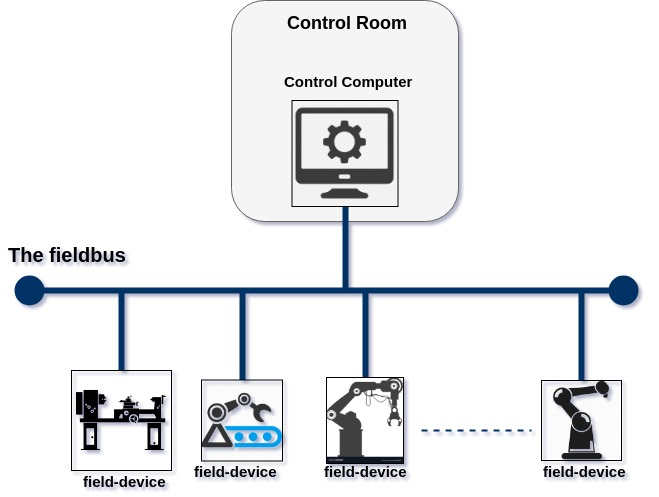
\includegraphics[width=9cm]{figures/fieldbus/fieldbus_network.jpg}
\caption{Fieldbus network}\label{fieldbus_network}
\end{figure}

\subsection{Industrial Ethernet}

Ethernet is a very important communication platform (a physical layer and a data link layer)
which was standardized by the \ac{IEEE} as IEEE 802.3 \cite{kunbusIndustrialEthernet}.
Ethernet is now the most popular and the most widely used network technology in the world which without
it, communication between devices in today’s modern world would not be possible. For instance, Ethernet
is used to connect devices in companies networks like printers and computers, to connect devices in
our houses, to connect servers, routers and plenty of other examples.

A key strength of Ethernet is that it enables to run many protocols simultaneously on the
same network also it provides flexibility and scalability in a way not seen before. With the
growth of Ethernet and having these advantages, the idea of using Ethernet in the industry was introduced.
This, in fact, enables a common communication platform for all industrial network protocols. Also, this makes possible to let the
field devices communicate with the office devices (using the \ac{TCP}/\ac{IP} model) which provides more
flexibility and scalability. Therefore, field devices control and monitoring are not only possible from
inside the plant, but also from outside. For instance, a web server could be installed on a field device
and could be accessed from an office device to monitor what is happening on the field level \cite{profinet2013ethernet}.

Unfortunately, when Ethernet was introduced, the transmission data rate was 10 Mbit/s which is not suitable for
industrial communication. This led to the development of what is called fast-Ethernet with transmission data
rates of 100 Mbit/s and 1 Gbit/s which is considered sufficient for industrial usage. Another issue is that
using Ethernet in the industry requires additional considerations not seen in Ethernet systems used in an
office. In fact devices in industrial environments are exposed to different temperatures, vibrations
and other potentially disturbing noises and movements \cite{kunbusIndustrialEthernet}.
% The wiring technology being used within Ethernet is RJ45
% which was developed for non-industrial communication. For this purpose, a new RJ45 with additional protection
% was developed in order to meet the requirements needed in industrial environments \cite{kunbusIndustrialEthernet}.

As we know, in industrial applications, the real-time performance highly matters and has a considerable effect on
the automated process. As we discussed previously, using Ethernet in the industry enables the communication
between the office devices and the field devices. This is, of course, possible using the \ac{TCP}/\ac{IP} communication model. Unfortunately, \ac{TCP}/\ac{IP}
could not be fast enough to satisfy some applications with tight and critical time requirements. In fact, when data is sent using  \ac{TCP}/\ac{IP}, like \autoref{data_encapsulation_for_non_critical_time_applications} shows, the data is packed
into the application layer then into the transport layer which basically \ac{TCP}   or \ac{UDP} then packed into \ac{IP} datagram and
finally into Ethernet frame. When the Ethernet frame is received, the previously cited layers need to be unpacked in
order to get the data. The operation of packing and unpacking data through several layers consumes a considerable amount
of time that's why alongside using \ac{TCP}/\ac{IP} another approach is commonly used in order meet the requirements of
critical-time applications. The idea behind this approach is basically to minimize the number of packing and unpacking
operations by skipping the network and transport layers (\ac{IP}  and \ac{TCP}   /\ac{UDP}) which significantly increases the
performance. The \autoref{data_encapsulation_for_critical_time_applications} illustrates the second approach \cite{profinet2013ethernet}.
\begin{figure}
\centering
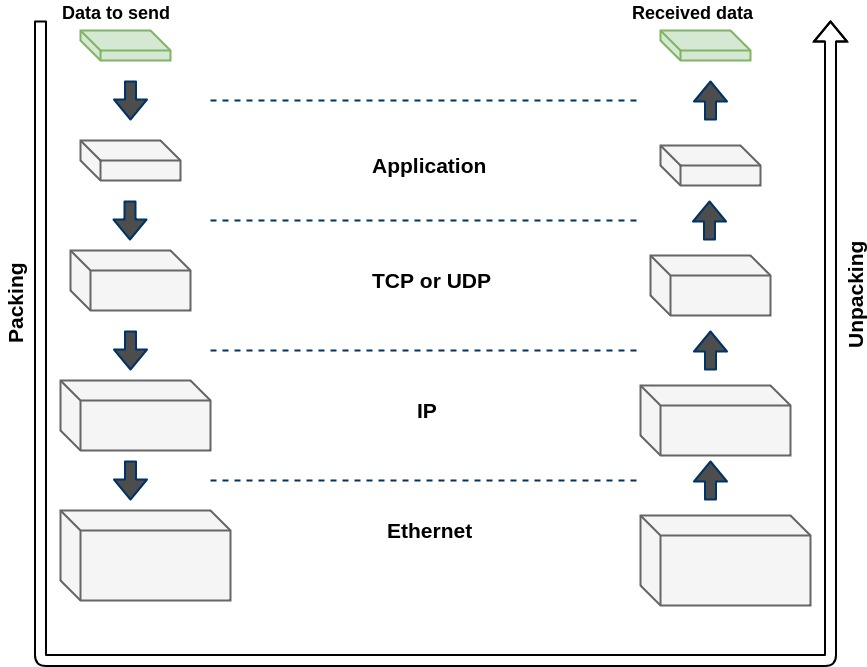
\includegraphics[width=12cm,height=8cm]{figures/indutrial_ethernet/data_encapsulation_for_non_critical_time_applications.jpg}
\caption{Data encapsulation for non-critical-time applications}\label{data_encapsulation_for_non_critical_time_applications}
\end{figure}

\begin{figure}
\centering
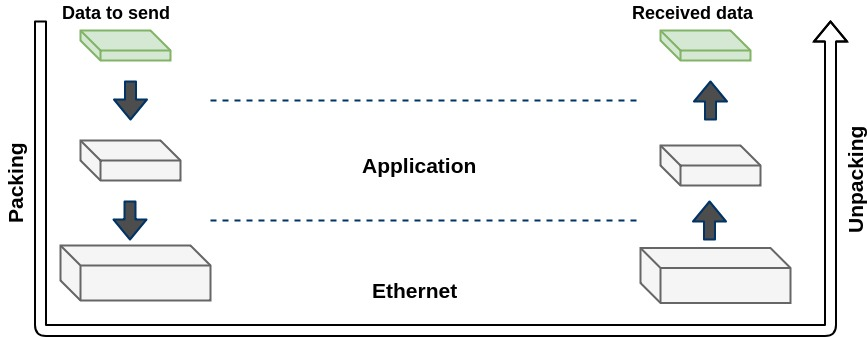
\includegraphics[width=12cm,height=6cm]{figures/indutrial_ethernet/data_encapsulation_for_critical_time_applications.jpg}
\caption{Data encapsulation for critical-time applications}\label{data_encapsulation_for_critical_time_applications}
\end{figure}

\section{SafetyNETp protocol}
\label{SafetyNETp}
SafetyNETp is a communication protocol developed by Pilz GmbH & Co. KG, which allows the
construction of industrial Ethernet-based networks and is suitable for both real-time communications and
safety-oriented applications. The meaning of safety does not refer to networking security, however, it
refers to safety applied to humans and to the environment. SafetyNETp is used wherever the temporal and content
consistency of communicated data is required to hedge dangers. The dangers can be the endangering of lives as well as the plant assets.
The second field of application is the communication of data in real time. With bus cycle times of
up to 62.5 microseconds, SafetyNETp can be used even in extremely time-critical areas.
Typical fields of application are factory automation (e.g. automobile production), transport
technology (e.g. cable cars). In general, all applications of automation and process technology are
possible \cite{KunbusSafetyNETp}.


The protocol enables the transmission of safety-related data on the same
cable used for the transfer of control or process data. In fact, it can
be used to transfer safety data without the need for a physical dedicated communication line.
Combining safe and nonsafe communications over the same medium have several advantages. First of
all, the reduced amount of cables needed to connect the network elements makes the wiring of components simpler, thus reducing costs for setup and maintenance. Moreover, the ability to connect safe
and nonsafe devices to the same network makes a number of non-safety-related functions (e.g. remote
diagnostic, data logging) available for safe devices and at the same time allows standard devices to
access safety data \cite{zurawski2014industrial}.

The communication mode commonly used in the industry is the Master/Slave mode. Within
this mode, the master can request to read a value from a slave or also write a value to it.
The slaves can't communicate directly with each other, they just respond to the read
requests sent by a given master and apply the received commands. Hence this mode
requires always a centralized controller. The \autoref{master-slave-mode} shows an example
of Master/Slave communication \cite{JonasFieldbus}.

\begin{figure}[H]
\centering
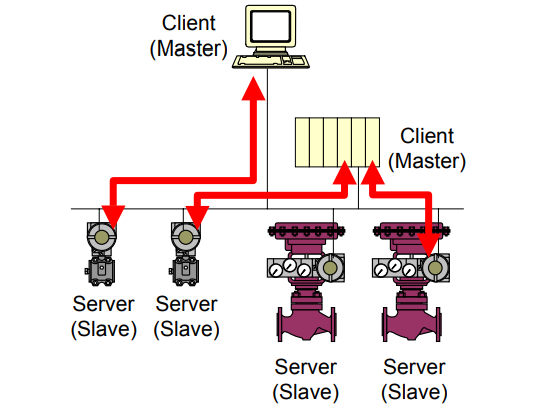
\includegraphics[width=10cm,height=4.6cm]{figures/safetynetp/master-slave-mode.png}
\caption[Master/Slave communication]{Master/Slave communication \cite{JonasFieldbus}}\label{master-slave-mode}
\end{figure}

In order to avoid the need for a centralized device and to make the data available to
all devices, SafetyNETp uses a multi-master bus system where all devices are given the same rights \cite{zurawski2014industrial}. It uses
a Publisher/Subscriber mode, where each device publishes its relevant data and can subscribe, at the same time,
the reception of data needed to carry out its tasks, which are produced by other entities in the network.
The \autoref{publish-subscribe-mode} shows an example of Publish/Subscribe communication.

\begin{figure}[H]
\centering
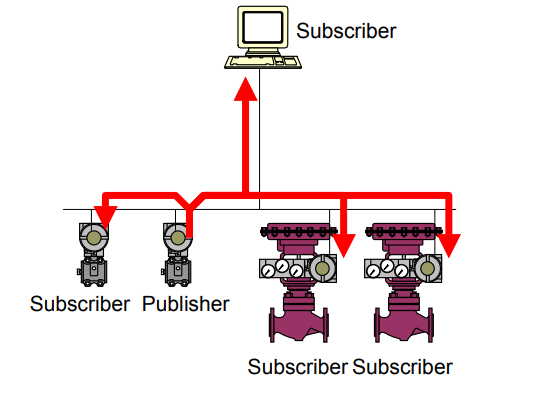
\includegraphics[width=10cm,height=6cm]{figures/safetynetp/publish-subscribe-mode.png}
\caption[Publish subscribe communication]{Publish subscribe communication \cite{JonasFieldbus}}\label{publish-subscribe-mode}
\end{figure}

As cited in the first chapter, SafetyNETp provides two communication models \ac{RTFN} and \ac{RTFL}. In the next sections, we present the
frame layout of both \ac{RTFN} and \ac{RTFL}, a brief overview about \ac{RTFN} and a detailed explanation of \ac{RTFN}.

\subsection{Frame layout}

As the \autoref{safetynetp_in_osi_model} shows, \ac{RTFN} runs on top of \ac{UDP} and \ac{RTFL} runs on top of Ethernet. Therefore \ac{RTFN}'s application
data represents \ac{UDP}'s payload and \ac{RTFL}'s application data represents Ethernet's payload. The SafetyNETp header is a one-byte
field which indicates the frame type or in other words the payload's content.

\begin{figure}[H]
\centering
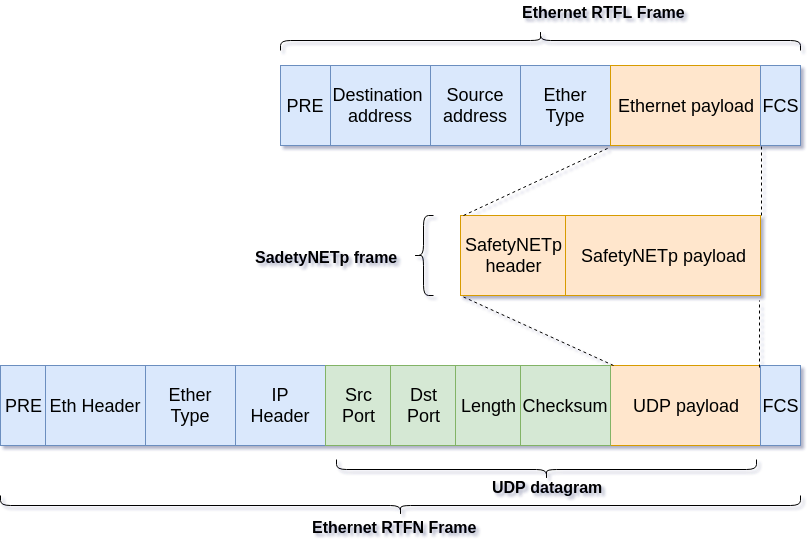
\includegraphics[width=10cm,height=8cm]{figures/safetynetp/safetynetp_frame_layout.png}
\caption{Mapping of SafetyNETp frame into Ethernet frame and UDP datagram}\label{frame-layout}
\end{figure}

\subsection{RTFL}

\ac{RTFL} has been designed for applications where real-time performance is of primary
importance. It is based on a linear topology, and the transport of data is supported through
standard Ethernet (OSI layer 2) frames. This communication model enables a minimum bus scan
time of 62.5 microsecond and limits jitters to 100 nanoseconds or less, making the protocol suitable for highly demanding
control applications \cite{zurawski2014industrial}. The reasoning behind skipping the network and the transport layers is to
increase the performance and this is achieved by reducing the time of packets processing (packing and unpacking).
\ac{RTFL} uses the linear topology which in fact keeps the advantages of Fieldbus systems. All devices are
connected through one single line which reduces the wiring costs and makes the data available for all devices.

As shown in \autoref{rtfl-physical-line}, in an \ac{RTFL} network, the communication is initiated by a special device called root device (RD). At each communication
cycle, the RD creates an \ac{RTFL} Ethernet frame and sends it along the line. All the cascading devices, also known as ordinary devices (ODs), append their data to the frame. When the frame reaches the end
of the line (last device), it is forwarded on the way back to the RD. While traveling in this direction, relevant
data are then read by the different ODs. Each \ac{RTFL} network requires just one RD.

\begin{figure}[H]
\centering
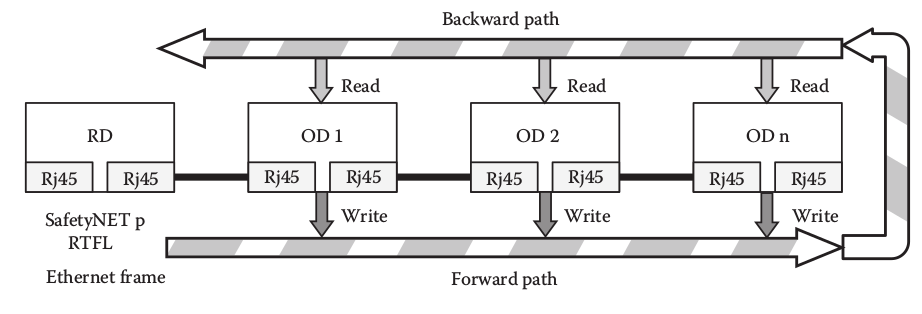
\includegraphics[width=10cm,height=5cm]{figures/safetynetp/rtfl-physical-line.png}
\caption{RTFL physical line}\label{rtfl-physical-line}
\end{figure}

\ac{RTFL} is designed to minimize the overhead by using frames as common containers for data from all devices.
As depicted in \autoref{rtfl-ethernet-frame} a single Ethernet frame can carry all process data needed by the devices. Minimizing the header overhead is important to reach
cycle times as short as 62.5 microseconds, which are needed especially in motion control applications.

\begin{figure}[H]
\centering
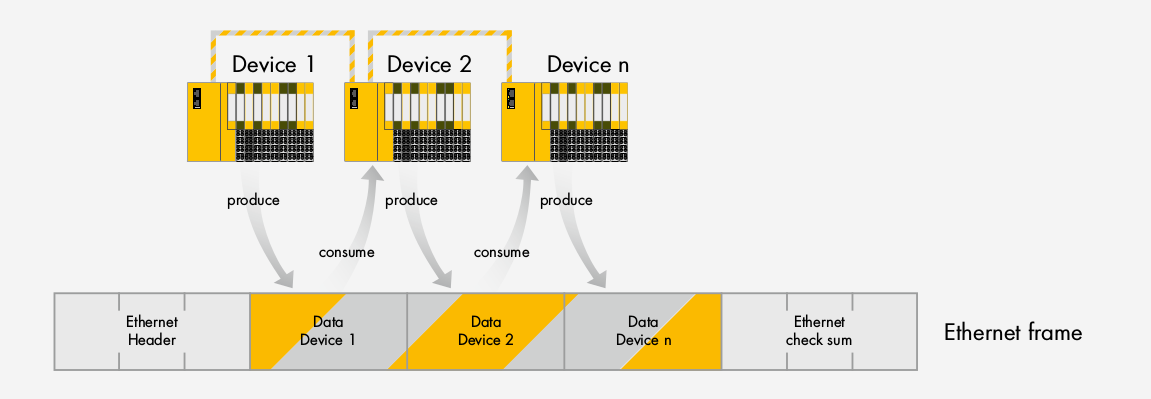
\includegraphics[width=15cm,height=5cm]{figures/safetynetp/rtfl-ethernet-frame.png}
\caption{RTFL Ethernet frame}\label{rtfl-ethernet-frame}
\end{figure}

\subsection{RTFN}

When real-time requirements are not so tight and a cycle time over 1 millisecond is sufficient, the \ac{RTFN} communication model
can be used to obtain the maximum degree of flexibility and integration with other
standard Ethernet-based protocols likely adopted at higher levels of the factory hierarchy. In fact, \ac{RTFN}
can use the standard \ac{UDP}/\ac{IP}  protocols to transport data, allowing both the routing of frames among
different networks and the integration with the existing communication infrastructures. \ac{RTFN}
can be used for communication between field devices and for connecting the field devices to
the office network. \ac{RTFN} is compatible with \ac{RTFL} and it can be used to connect multiple \ac{RTFL} networks together.
\ac{RTFN} does not restrict the usage of a specific topology, it allows using any network topology, for
instance, star, tree and ring topologies.

\ac{RTFN} follows a Publish/Subscribe communication model where the data is exchanged through
the concept of topics. An \ac{RTFN} device could be a publisher, a subscriber or both together.
Each publisher has a list of topics. When a publisher receives a \textit{subscribe request} for a topic it has,
it responds by sending data about the subscribed topic to the subscriber and this is called publishment.
For instance, a temperature sensor could be a publisher which has the temperature as a topic. A device
could get the temperature value by subscribing to the corresponding topic.
In an \ac{RTFN} network, as it is shown in \autoref{rtfn-frame-and-messages-type}, six types of messages
could be exchanged between devices:
\begin{itemize}
\setlength{\labelwidth}{10pt}
  \item Subscribe request: used by subscribers to request the subscription for a specific topic.
  \item Subscribe acknowledgment: used by a publisher to confirm that a subscription request has been accepted.
  \item Unsubscribe request: used by a subscriber to unsubscribe the reception of some topic.
  \item Still alive: sent by a subscriber to a publisher to inform it that it is still alive.
  \item Unpublished: sent by a publisher to a subscriber to inform it that no more data will be received for a certain topic.
  \item Cyclic data: message sent cyclically by the publisher to the subscriber which contains topics' data.
\end{itemize}

\begin{figure}[H]
\centering
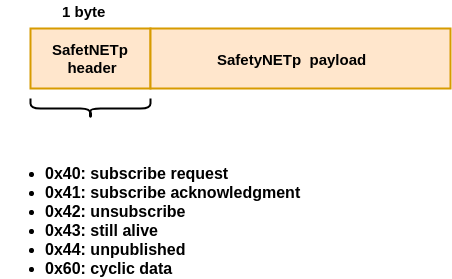
\includegraphics[width=10cm,height=4cm]{figures/safetynetp/rtfn-frame-and-messages-type.png}
\caption{RTFN frame and messages type}\label{rtfn-frame-and-messages-type}
\end{figure}

The sequence diagram shown in \autoref{rtfn-pub-sub} illustrates the subscription and the publishment process. In this
diagram, for simplicity reasons, we assume that the messages are sent reliably (no message loss). The publisher and the
subscriber don't know each other in advance, that's why the subscriber starts by sending a \textit{subscribe request} as broadcast (the \textit{subscribe request}
will be sent to all the devices in the network). The devices present in the network will receive the \textit{subscribe request} and
the device which has the topic available will send back a \textit{subscribe acknowledgment} as unicast to the subscriber.
Once the subscription process has finished, the publisher starts publishing cyclically data about the corresponding topic to the subscriber.
The published data is called \textit{cyclic data} and sent only to the subscriber. The subscriber also
sends cyclic messages to the publisher. These messages consist of \textit{still alive} messages that are sent in order to inform the publisher that the subscriber is still alive.

\begin{figure}[H]
\centering
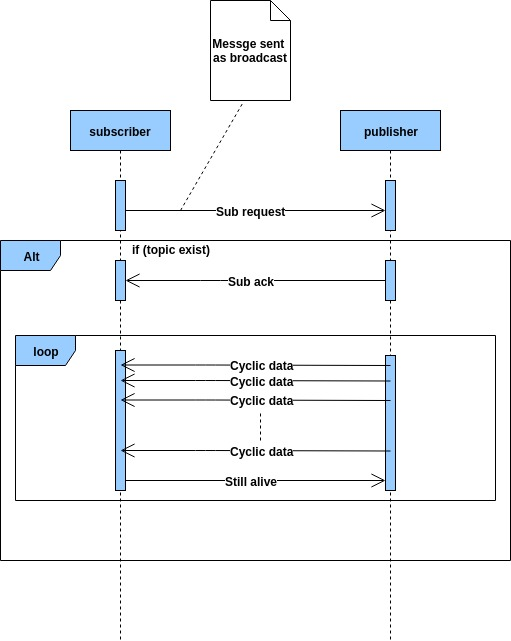
\includegraphics[width=10cm,height=9cm]{figures/safetynetp/rtfn-pub-sub.jpg}
\caption{RTFN Publish/Subscribe communication}\label{rtfn-pub-sub}
\end{figure}

The publisher can stop sending \textit{cyclic data} to the subscriber for multiple reasons.
If the subscriber is down, the publisher will not receive anymore \textit{still alive} messages, therefore
it will stop sending \textit{cyclic data}.
The subscriber can send an \textit{unsubscribe request} to the publisher in order to inform it that the cyclic
data for some topic is not needed anymore. The publisher will stop sending \textit{cyclic data} upon receiving the \textit{unsubscribe request}, moreover,
the publisher also can send an \textit{unpublished} message to the subscriber to inform it that no more \textit{cyclic data} will be published
for a certain topic.

For simplicity reasons, we assumed that there is no message loss. However as we mentioned before,
\ac{RTFN} uses \ac{UDP} as a transport layer which does not provide reliable transfer. What will happen if for
example the \textit{subscribe acknowledgment} sent by the publisher is lost? In fact, the subscriber will keep
sending always \textit{subscribe requests} until receiving a \textit{subscribe acknowledgment} from the publisher.

\section{Security Protocols}

In today's internet, almost everything is based on the \ac{TCP}/\ac{IP} model. The internet was primarily a small network
connecting a community of researchers, but with the success of \ac{TCP}/\ac{IP} the internet expanded to become a gigantic global
network connecting devices of all types. With the huge success of \ac{TCP}/\ac{IP} and the growth of the internet, \ac{TCP}/\ac{IP} application
became attractive for the industry and the automation area (e.g. Industrial Ethernet).
However, no security measures were taken into consideration while designing \ac{TCP}/\ac{IP} as it was only for
interconnecting small and private networks. In this section, we discuss the most common \ac{IP} security
measures.

\subsection{Secure Sockets Layer/Transport Layer Security}

% Today with the growth of the internet, we can do a lot of things from our mobile phones or PCs.
% We are able to send e-mails, files, photos and share all kind of data between our devices. We can
% buy products or even it's possible to perform money transactions through the internet. With the introduction of IoT,
% one can speak about smart houses. Everything in our houses can be commanded remotely. It
% is good to have all these services, unfortunately, without security measures, it can lead to
% crucial problems. That's why SSL/\ac{TLS} (Secure Sockets Layer/Transport Layer Security) protocol was introduced to solve the security problems.

\ac{SSL}/\ac{TLS} is the most widely deployed protocol for
securing network traffic. It is widely used for protecting Web traffic and for e-mail protocols such as
Internet Message Access Protocol (IMAP) and Post Office Protocol (POP). \ac{TLS} is developed for any reliable transport
protocol which maintains the messages' order. It is typically used for securing \ac{TCP} applications (e.g. HTTP).

\subsubsection{Introduction and History}

The first \ac{SSL} version was introduced by Netscape in 1994. In 1995 and 1996, \ac{SSL} versions 2.0 and 3.0 were released
and then came the release of \ac{TLS} 1.0 which is, in fact, the same as \ac{SSL} 3.1. Basically, there is no
difference between \ac{TLS} and SSL, beginning from \ac{SSL} version 3.1, the protocol name has been changed
to become \ac{TLS} 1.0 \cite{SSLHistory}. The last standardized \ac{TLS} version today is 1.2 which was released in 2008 in RFC5246 \cite{rfc5246}
, moreover, drafts are available for \ac{TLS} version 1.3. The last published draft of \ac{TLS} 1.3 was on 20 March 2018 \cite{draftTLSv1.3}.

The goal of SSL/\ac{TLS} is to provide the three crucial security services:

\begin{itemize}
\setlength{\labelwidth}{10pt}
  \item Confidentiality: the data is sent encrypted and only the devices which have the keying material could decrypt and read the data.
  The encryption is performed via symmetric encryption algorithms such as \ac{DES} or \ac{AES}.

  \item Integrity: communication partners can detect changes to a message during transmission.
  this is achieved using \ac{MAC}.

  \item Authentication: the recipient of a message can identify its communication
partner and can detect if the received message has been forged. The authentication
is likely based on a pre-shared key or on client's and server's certificates.
\end{itemize}

\ac{TLS} is based on a sub-protocol named record layer protocol which on
top of it we can find four protocols, the Handshake protocol, the Change Cipher Spec protocol,
the Alert protocol and the Application Data protocol (\autoref{tls-protocol-architecture}). Among these four protocols, the most
important one is the Handshake protocol which is used for establishing an authenticated
cryptographic secret between two endpoints by commonly using public key cryptography \cite{rfc5246}.

\begin{figure}[H]
\centering
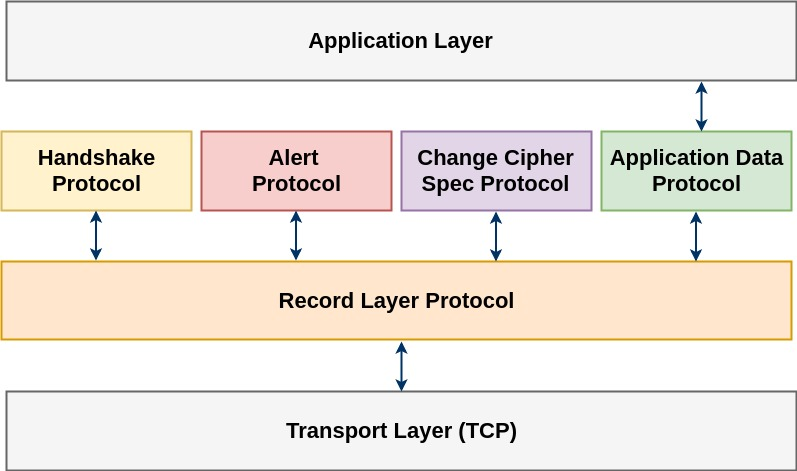
\includegraphics[width=10cm,height=6cm]{figures/dtls/tls-protocol-architecture.jpg}
\caption{TLS protocol architecture}\label{tls-protocol-architecture}
\end{figure}

\subsubsection{\ac{TLS} Handshake}

\ac{TLS} is designed to work on top of a reliable transport protocol typically \ac{TCP}. It follows the Client/Server
communication model and its goal is to establish a secure connection between a server and a client
and let them exchange data securely across an untrusted network. To establish a secure connection, the \ac{TLS} handshake needs to take
place. During the handshake, important messages are exchanged between the client and the server. With the messages exchanged
the client and the server basically agree on the protocol version, select the encryption and the MAC algorithms,
authenticate each other by exchanging and validating digital certificates and share a symmetric encryption key to be used
for encryption \cite{rfc5246}.

\begin{figure}[!htbp]
\centering
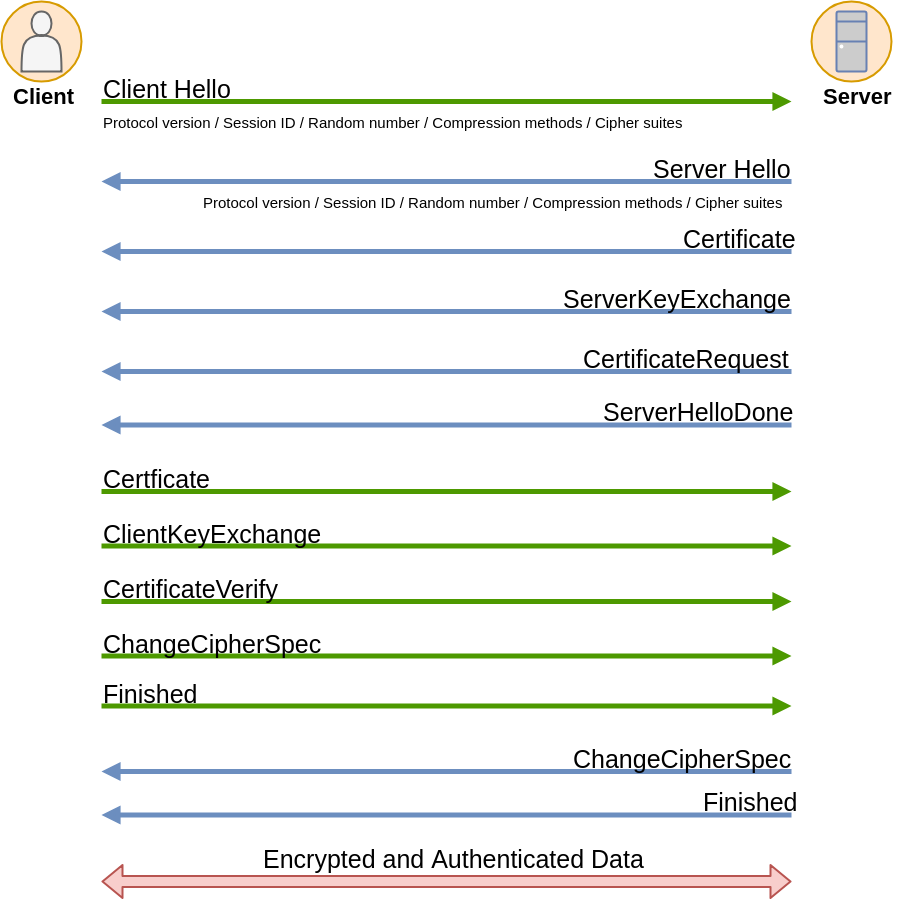
\includegraphics[width=11cm,height=14cm]{figures/dtls/tls-handshake.png}
\caption{SSL/TLS full handshake}\label{tls-handshake}
\end{figure}


As standardized in RFC5246 \cite{rfc5246}, a full SSL/\ac{TLS} handshake contains the following messages (\autoref{tls-handshake}):

\begin{itemize}
\setlength{\labelwidth}{10pt}
  \item Client Hello: it is the first handshake message and it is sent from the client to the server.
  It contains the supported \ac{SSL} and \ac{TLS} versions, a random number, a session id and the supported compression methods and cipher suites. In fact, cipher suites are very important
  as they define the key exchange algorithm, the authentication algorithm (digital signature algorithm),
  the data encryption algorithm as well as the MAC algorithm (\autoref{tls-cipher-suite-example}).

  \begin{figure}[H]
  \centering
  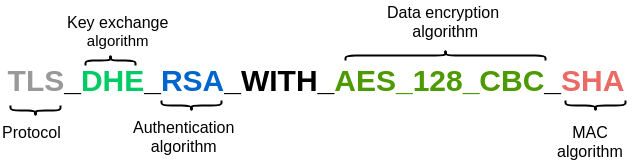
\includegraphics[width=10cm,height=2.5cm]{figures/dtls/tls-cipher-suite-example.png}
  \caption{TLS cipher suite example}\label{tls-cipher-suite-example}
  \end{figure}

  \item Server Hello: upon receiving the Client Hello, the server sends back the Server Hello message
  which contains the selected parameters (key exchange algorithm, the authentication algorithm...).

  \item Server Certificate: it is optional to send, it lets the client verify the identity of the server.

  \item Server Key Exchange: this message is not always present in the handshake, it is only sent if
  the server certificate is not sufficient to allow the client to exchange the secret key.

  \item Certificate Request: it is optional to send, it informs the client to provide its certificate
  for authentication.

  \item Server Hello Done: sent by the server to indicate the end of the Server Hello and the associated messages
  (Server Certificate, Server Key Exchange, and Certificate Request). Upon receiving the Server Hello done, the client verifies the validity of the server certificate and the parameters selected by the server in the Server Hello.

  \item Client Key Exchange: it is sent by the client after receiving the Server Hello Done to set the \ac{PMS}. The content of this messages depends on the selected key exchange algorithm, if RSA is chosen,
  the PMS is encrypted against the server's public key, however, if \ac{DH} is chosen, DH parameters will be sent. The PMS secret will be used on both sides to compute a shared \ac{MS} which will be used for encryption, decryption and MAC calculation.

  \item Client Certificate: sent if required by the server, it allows the server to verify the identity of the client.

  \item Certificate Verify: if the client sends a certificate with signing ability, a digitally-signed Certificate Verify message is sent in order to explicitly verify the certificate.

  \item Change Cipher Spec: sent by both the client and the server. This message indicates that the following messages
  will be sent encrypted using the shared keying material.

  \item Finished: sent by both the client and the server after the Change Cipher Spec message to verify that the key exchange and authentication processes were successful. It is the last handshake message and the first encrypted one.

\end{itemize}


\subsubsection{How the security services are ensured?}

In our project, when we say security services, we mean basically confidentiality, integrity, and authenticity.
When the server sends its certificate, the client verifies the validity of the certificate using the public key of the
\ac{CA}. If the certificate is valid, the client generates a PMS and sends it to the server.
Not only the client can verify the server identity, also the server verifies the client identity, in the same way, using
the client certificate. If the client certificate is valid the server will accept the provided PMS.
Using the PMS, both the client and server derive a MS which is in turn used to derive other several keys.
These keys are used for exchanging authenticated and encrypted data with the capability to the check its integrity.
The confidentiality is ensured by encrypting the data, the authentication and the integrity are both ensured using a MAC algorithm \cite{rfc5246}.


\subsection{Datagram Transport Layer Security}

A lot of applications today in several domains are delay sensitive and have tight time constraints.
For instance, we can speak of industrial communication, IoT, internet telephony, online gaming and several other applications.
Due to the time constraints, for this kind of applications \ac{UDP} is used instead of \ac{TCP}   .

\subsubsection{Introduction and History}

Application layer protocols that work on top of \ac{TCP} such as Hypertext Transfer
Protocol (HTTP), Secure Shell (SSH) or File Transfer Protocol (FTP) can be easily secured using
\ac{TLS} as it is designed to secure applications working on top of a reliable transport protocol. Unfortunately,
for datagram based applications, no such alternative exists. Therefore, similarly to TLS, DTLS
was introduced to allow the use of the same security services provided by \ac{TLS} but for datagram based applications.

Over the years, \ac{TLS} has become more robust and has been refined to withstand numerous attacks that's why
\ac{DTLS} was designed to be as similar as possible to it. By minimizing the changes, the risk of introducing new weaknesses
or vulnerabilities will be reduced. Moreover, \ac{DTLS} implementation will be easier by reusing \ac{TLS} pre-existing infrastructure \cite{designAndImlementationOfDTLS}.

The last standardized \ac{DTLS} version is 1.2, it was standardized in 2012 as RFC6347 \cite{rfc6347}. Like TLS,
drafts have been published for \ac{DTLS} version 1.3. The last draft was published on 02 July 2018 \cite{draftDTLSv1.3}.

\subsubsection{\ac{DTLS} Design}

\ac{TCP}   provides a reliable bi-directional tunnel for bytes, where all bytes eventually reach the receiver
in the same order as what the sender used to send them. \ac{TCP} achieves that through a complex
assembly of acknowledgment messages, transmission timeouts and retransmission. As \ac{TLS} uses \ac{TCP},
it does not encounter issues related to packet loss and reordering which is not the case for DTLS.

The unreliability of datagram protocols creates problems for \ac{TLS} in two levels.
First, the messages decryption is dependent from the previous messages as the integrity check is based on the
implicit sequence number. If record N is not received, then the integrity check
on record N+1 will be based on the wrong sequence number and
thus will fail. Second, \ac{TLS} assumes that the handshake messages are sent reliably, hence,
the connection cannot be established if a handshake message is lost \cite{rfc5246}.

In order to handle packet loss, \ac{DTLS} uses a retransmission timer described in details in RFC6347 \cite{rfc6347}.
\ac{DTLS} includes an explicit sequence number which is used
for MAC calculation. It is used also to detect replay attacks and reordering. Furthermore, a new field was introduced named epoch which is incremented each time a CipherChangeSpec
message is sent.

Some \ac{TLS} cipher suites retain a cryptographic context between records which
does not allow to process individual records. This will cause problems with
unreliable protocols, therefore, \ac{DTLS} banned the usage of this kind of cipher suites \cite{rfc5246}.

\ac{TLS} and \ac{DTLS} handshakes are the same except that \ac{DTLS} has introduced a new message which does not
exist in \ac{TLS}'s handshake. The new message is named Hello Verify Request, it contains a cookie and it is sent back
to the client just after receiving the Client Hello message. the client should send back another Client Hello
which contains the same cookie. If the cookie is verified the handshake will continue (same \ac{TLS} handshake steps), otherwise,
the server will close the connection. The cookie mechanism allows reducing the risk of \ac{DoS} attacks.
No such message exists in \ac{TLS} handshake because the \ac{TCP}   handshake is established before starting the \ac{TLS} handshake
which will make the DoS attack difficult. This is not the case for datagram protocols because no connection is established prior to
the \ac{DTLS} handshake, hence, the cookie mechanism is needed \cite{rfc6347}.

\subsection{Internet Protocol Security}

\ac{IPsec} is a protocol suite which was introduced to secure network traffic and more specifically \ac{IP} and its
upper layers protocols, typically \ac{TCP} or \ac{UDP}. \ac{IPsec} is situated in layer three of the OSI model and it offers data
integrity, replay protection, authentication, and confidentiality natively within the \ac{IP} layer. \ac{IPsec}
offers two communication modes, tunnel mode and transport mode (\autoref{ipsec_communication_modes}).
The tunnel mode provides network-to-network security whereas the transport mode provides host-to-host security.
In fact, in the tunnel mode, the sender sends the message as it is (unprotected) to the gateway, then the gateway encapsulates the message
and sends it securely. The receiving gateway decapsulates the secured message and passes the original message to the receiver if
the message is verified correctly (e.g. integrity, authentication). In the transport mode, unlike the tunnel mode, protecting
the messages is no longer performed by the gateway, instead, the end hosts manage themselves to secure and verify the messages.

 \begin{figure}[!htbp]
 \centering
 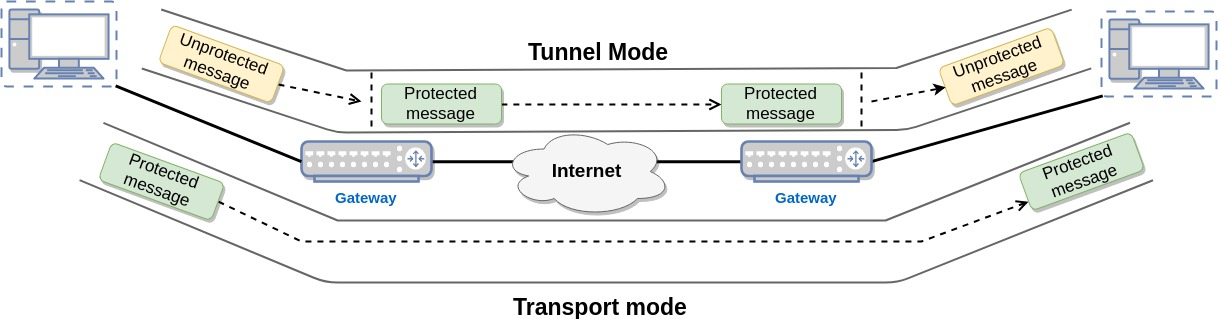
\includegraphics[width=16cm]{figures/IPsec/ipsec_modes.jpg}
 \caption{IPsec communication modes}\label{ipsec_communication_modes}
 \end{figure}

 To provide its security services, \ac{IPsec} use three independent protcols:

 \begin{itemize}
 \setlength{\labelwidth}{10pt}
   \item \ac{AH}: It provides integrity and authentication for the \ac{IP} header and its payload in both tunnel and transport modes and optionally provides protection against replay attacks. However, it does not provide confidentiality. The \ac{IP} header mutable fields (the fields which can change during the transmission) like
   \ac{TTL} are not authenticated.
   \item \ac{ESP}: It provides confidentiality, integrity, and authentication for the \ac{IP} payload in both modes.
   However, it does not provide protection for the \ac{IP} header.
   \item \ac{IKE}: It allows to share an authenticated secret key to be used for encryption, authentication, and integrity checks.
   it uses DH as a key exchange algorithm and RSA for digital signatures.
 \end{itemize}

 As depicted in \autoref{ipsec_protocols}, whether \ac{AH} or \ac{ESP} is adopted, if the tunnel mode is used, when the gateway receives the original \ac{IP} datagram from the sender,
 it encapsulates it into a new \ac{IP} datagram containing a new \ac{IP} address which corresponds to the receiving gateway and then the message is protected. When the transport mode is used the original \ac{IP} datagram is protected by the sender and sent without new \ac{IP} encapsulation.
 \ac{ESP} and \ac{AH} could be used separately or together according to the needed security services.


 \begin{figure}[!htbp]
 \centering
 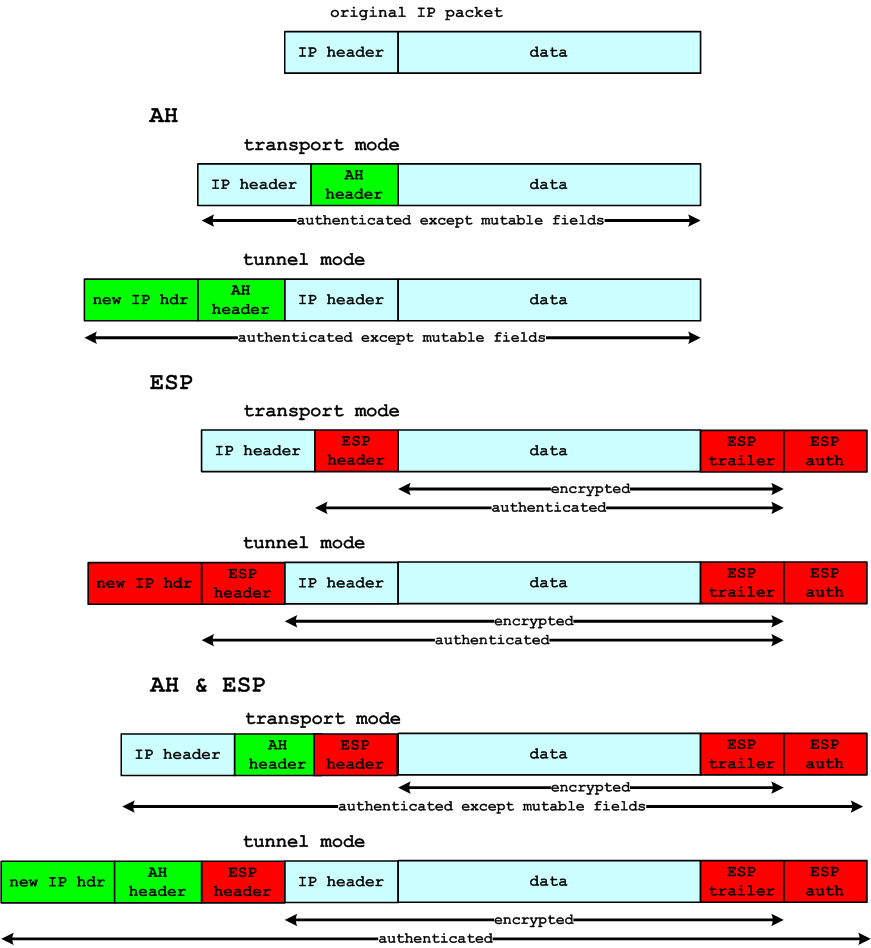
\includegraphics[width=16cm]{figures/IPsec/ipsec_protocols.png}
 \caption{IPsec protocols}\label{ipsec_protocols}
 \end{figure}

\section{Choice of Security Protocol}

We need to take into consideration first that SafetyNETp \ac{RTFN} works on top of \ac{UDP}.
\ac{DTLS} and \ac{TLS} provide the same security services. \ac{TLS} is used for reliable transport protocols whereas DTLS
is for unreliable ones. \ac{IPsec} can be used for securing any type of traffic working on top \ac{IP}.
Therefore our choice is restricted between \ac{DTLS} and \ac{IPsec}.

Automation systems and their real-time operating
systems often are resource constrained and do not include typical security technologies,
and there may not be available computing resources to retrofit these security technologies. \ac{IPsec} tunnel mode
is a solution as the cryptographic operations are performed by the gateways. The end devices send and receive the messages transparently, no additional treatment is needed for them. However, the tunnel mode protects the network only from outside because
messages exchanged on the local network are not secured by the gateway. Hence, we could have serious problems if
an attacker gains access to the local network. \ac{IPsec} transport mode provides end-to-end security and allows to secure the network both
from inside and outside, however, the cryptographic operations are done by the end devices which have constrained resources.
\ac{IPsec} operates at the \ac{IP} layer, it generally must be implemented in the operating
system kernel, either directly compiled in or linked in as a loadable module. This makes \ac{IPsec} fairly inconvenient
to install on non-\ac{IPsec} systems. \ac{AH} and \ac{ESP} are typically implemented in the kernel as part of the \ac{IP} stack, while \ac{IKE}
is implemented as a user daemon. This makes its integration difficult as most of the embedded \ac{IP} stacks do not implement \ac{IPsec}.

\ac{DTLS} provides end-to-end security and like \ac{IPsec}, the cryptographic operations are performed by the end devices.
\ac{DTLS} operates between the transport layer and the application layer. Using DTLS, it is easy to secure an application
 protocol by simply inserting it between the application and the transport layers. \ac{DTLS} is \ac{IP}-stack-independent
which means that it does not include any modification to the underlying \ac{IP} stack and could be used with any \ac{IP} stack implementation,
hence, its integration in embedded \ac{IP} stacks is a lot easier.

Having that Both, \ac{IPsec} and \ac{DTLS} provide the needed security services (confidentiality, integrity, and authentication),
and based on the previous paragraphs, we decide to use DTLS.

\section*{Conclusion}

After going through the necessary concepts needed for our project, in the next chapter, we go through a
brief security analysis and we present the functional and non-functional requirements.
